
% Default to the notebook output style

    


% Inherit from the specified cell style.




    
\documentclass[11pt]{article}

    
    
    \usepackage[T1]{fontenc}
    % Nicer default font (+ math font) than Computer Modern for most use cases
    \usepackage{mathpazo}

    % Basic figure setup, for now with no caption control since it's done
    % automatically by Pandoc (which extracts ![](path) syntax from Markdown).
    \usepackage{graphicx}
    % We will generate all images so they have a width \maxwidth. This means
    % that they will get their normal width if they fit onto the page, but
    % are scaled down if they would overflow the margins.
    \makeatletter
    \def\maxwidth{\ifdim\Gin@nat@width>\linewidth\linewidth
    \else\Gin@nat@width\fi}
    \makeatother
    \let\Oldincludegraphics\includegraphics
    % Set max figure width to be 80% of text width, for now hardcoded.
    \renewcommand{\includegraphics}[1]{\Oldincludegraphics[width=.8\maxwidth]{#1}}
    % Ensure that by default, figures have no caption (until we provide a
    % proper Figure object with a Caption API and a way to capture that
    % in the conversion process - todo).
    \usepackage{caption}
    \DeclareCaptionLabelFormat{nolabel}{}
    \captionsetup{labelformat=nolabel}

    \usepackage{adjustbox} % Used to constrain images to a maximum size 
    \usepackage{xcolor} % Allow colors to be defined
    \usepackage{enumerate} % Needed for markdown enumerations to work
    \usepackage{geometry} % Used to adjust the document margins
    \usepackage{amsmath} % Equations
    \usepackage{amssymb} % Equations
    \usepackage{textcomp} % defines textquotesingle
    % Hack from http://tex.stackexchange.com/a/47451/13684:
    \AtBeginDocument{%
        \def\PYZsq{\textquotesingle}% Upright quotes in Pygmentized code
    }
    \usepackage{upquote} % Upright quotes for verbatim code
    \usepackage{eurosym} % defines \euro
    \usepackage[mathletters]{ucs} % Extended unicode (utf-8) support
    \usepackage[utf8x]{inputenc} % Allow utf-8 characters in the tex document
    \usepackage{fancyvrb} % verbatim replacement that allows latex
    \usepackage{grffile} % extends the file name processing of package graphics 
                         % to support a larger range 
    % The hyperref package gives us a pdf with properly built
    % internal navigation ('pdf bookmarks' for the table of contents,
    % internal cross-reference links, web links for URLs, etc.)
    \usepackage{hyperref}
    \usepackage{longtable} % longtable support required by pandoc >1.10
    \usepackage{booktabs}  % table support for pandoc > 1.12.2
    \usepackage[inline]{enumitem} % IRkernel/repr support (it uses the enumerate* environment)
    \usepackage[normalem]{ulem} % ulem is needed to support strikethroughs (\sout)
                                % normalem makes italics be italics, not underlines
    

    
    
    % Colors for the hyperref package
    \definecolor{urlcolor}{rgb}{0,.145,.698}
    \definecolor{linkcolor}{rgb}{.71,0.21,0.01}
    \definecolor{citecolor}{rgb}{.12,.54,.11}

    % ANSI colors
    \definecolor{ansi-black}{HTML}{3E424D}
    \definecolor{ansi-black-intense}{HTML}{282C36}
    \definecolor{ansi-red}{HTML}{E75C58}
    \definecolor{ansi-red-intense}{HTML}{B22B31}
    \definecolor{ansi-green}{HTML}{00A250}
    \definecolor{ansi-green-intense}{HTML}{007427}
    \definecolor{ansi-yellow}{HTML}{DDB62B}
    \definecolor{ansi-yellow-intense}{HTML}{B27D12}
    \definecolor{ansi-blue}{HTML}{208FFB}
    \definecolor{ansi-blue-intense}{HTML}{0065CA}
    \definecolor{ansi-magenta}{HTML}{D160C4}
    \definecolor{ansi-magenta-intense}{HTML}{A03196}
    \definecolor{ansi-cyan}{HTML}{60C6C8}
    \definecolor{ansi-cyan-intense}{HTML}{258F8F}
    \definecolor{ansi-white}{HTML}{C5C1B4}
    \definecolor{ansi-white-intense}{HTML}{A1A6B2}

    % commands and environments needed by pandoc snippets
    % extracted from the output of `pandoc -s`
    \providecommand{\tightlist}{%
      \setlength{\itemsep}{0pt}\setlength{\parskip}{0pt}}
    \DefineVerbatimEnvironment{Highlighting}{Verbatim}{commandchars=\\\{\}}
    % Add ',fontsize=\small' for more characters per line
    \newenvironment{Shaded}{}{}
    \newcommand{\KeywordTok}[1]{\textcolor[rgb]{0.00,0.44,0.13}{\textbf{{#1}}}}
    \newcommand{\DataTypeTok}[1]{\textcolor[rgb]{0.56,0.13,0.00}{{#1}}}
    \newcommand{\DecValTok}[1]{\textcolor[rgb]{0.25,0.63,0.44}{{#1}}}
    \newcommand{\BaseNTok}[1]{\textcolor[rgb]{0.25,0.63,0.44}{{#1}}}
    \newcommand{\FloatTok}[1]{\textcolor[rgb]{0.25,0.63,0.44}{{#1}}}
    \newcommand{\CharTok}[1]{\textcolor[rgb]{0.25,0.44,0.63}{{#1}}}
    \newcommand{\StringTok}[1]{\textcolor[rgb]{0.25,0.44,0.63}{{#1}}}
    \newcommand{\CommentTok}[1]{\textcolor[rgb]{0.38,0.63,0.69}{\textit{{#1}}}}
    \newcommand{\OtherTok}[1]{\textcolor[rgb]{0.00,0.44,0.13}{{#1}}}
    \newcommand{\AlertTok}[1]{\textcolor[rgb]{1.00,0.00,0.00}{\textbf{{#1}}}}
    \newcommand{\FunctionTok}[1]{\textcolor[rgb]{0.02,0.16,0.49}{{#1}}}
    \newcommand{\RegionMarkerTok}[1]{{#1}}
    \newcommand{\ErrorTok}[1]{\textcolor[rgb]{1.00,0.00,0.00}{\textbf{{#1}}}}
    \newcommand{\NormalTok}[1]{{#1}}
    
    % Additional commands for more recent versions of Pandoc
    \newcommand{\ConstantTok}[1]{\textcolor[rgb]{0.53,0.00,0.00}{{#1}}}
    \newcommand{\SpecialCharTok}[1]{\textcolor[rgb]{0.25,0.44,0.63}{{#1}}}
    \newcommand{\VerbatimStringTok}[1]{\textcolor[rgb]{0.25,0.44,0.63}{{#1}}}
    \newcommand{\SpecialStringTok}[1]{\textcolor[rgb]{0.73,0.40,0.53}{{#1}}}
    \newcommand{\ImportTok}[1]{{#1}}
    \newcommand{\DocumentationTok}[1]{\textcolor[rgb]{0.73,0.13,0.13}{\textit{{#1}}}}
    \newcommand{\AnnotationTok}[1]{\textcolor[rgb]{0.38,0.63,0.69}{\textbf{\textit{{#1}}}}}
    \newcommand{\CommentVarTok}[1]{\textcolor[rgb]{0.38,0.63,0.69}{\textbf{\textit{{#1}}}}}
    \newcommand{\VariableTok}[1]{\textcolor[rgb]{0.10,0.09,0.49}{{#1}}}
    \newcommand{\ControlFlowTok}[1]{\textcolor[rgb]{0.00,0.44,0.13}{\textbf{{#1}}}}
    \newcommand{\OperatorTok}[1]{\textcolor[rgb]{0.40,0.40,0.40}{{#1}}}
    \newcommand{\BuiltInTok}[1]{{#1}}
    \newcommand{\ExtensionTok}[1]{{#1}}
    \newcommand{\PreprocessorTok}[1]{\textcolor[rgb]{0.74,0.48,0.00}{{#1}}}
    \newcommand{\AttributeTok}[1]{\textcolor[rgb]{0.49,0.56,0.16}{{#1}}}
    \newcommand{\InformationTok}[1]{\textcolor[rgb]{0.38,0.63,0.69}{\textbf{\textit{{#1}}}}}
    \newcommand{\WarningTok}[1]{\textcolor[rgb]{0.38,0.63,0.69}{\textbf{\textit{{#1}}}}}
    
    
    % Define a nice break command that doesn't care if a line doesn't already
    % exist.
    \def\br{\hspace*{\fill} \\* }
    % Math Jax compatability definitions
    \def\gt{>}
    \def\lt{<}
    % Document parameters
    \title{Assignment 2 - Function Approximation and using Neural Networks}
    
    
    

    % Pygments definitions
    
\makeatletter
\def\PY@reset{\let\PY@it=\relax \let\PY@bf=\relax%
    \let\PY@ul=\relax \let\PY@tc=\relax%
    \let\PY@bc=\relax \let\PY@ff=\relax}
\def\PY@tok#1{\csname PY@tok@#1\endcsname}
\def\PY@toks#1+{\ifx\relax#1\empty\else%
    \PY@tok{#1}\expandafter\PY@toks\fi}
\def\PY@do#1{\PY@bc{\PY@tc{\PY@ul{%
    \PY@it{\PY@bf{\PY@ff{#1}}}}}}}
\def\PY#1#2{\PY@reset\PY@toks#1+\relax+\PY@do{#2}}

\expandafter\def\csname PY@tok@gd\endcsname{\def\PY@tc##1{\textcolor[rgb]{0.63,0.00,0.00}{##1}}}
\expandafter\def\csname PY@tok@gu\endcsname{\let\PY@bf=\textbf\def\PY@tc##1{\textcolor[rgb]{0.50,0.00,0.50}{##1}}}
\expandafter\def\csname PY@tok@gt\endcsname{\def\PY@tc##1{\textcolor[rgb]{0.00,0.27,0.87}{##1}}}
\expandafter\def\csname PY@tok@gs\endcsname{\let\PY@bf=\textbf}
\expandafter\def\csname PY@tok@gr\endcsname{\def\PY@tc##1{\textcolor[rgb]{1.00,0.00,0.00}{##1}}}
\expandafter\def\csname PY@tok@cm\endcsname{\let\PY@it=\textit\def\PY@tc##1{\textcolor[rgb]{0.25,0.50,0.50}{##1}}}
\expandafter\def\csname PY@tok@vg\endcsname{\def\PY@tc##1{\textcolor[rgb]{0.10,0.09,0.49}{##1}}}
\expandafter\def\csname PY@tok@vi\endcsname{\def\PY@tc##1{\textcolor[rgb]{0.10,0.09,0.49}{##1}}}
\expandafter\def\csname PY@tok@mh\endcsname{\def\PY@tc##1{\textcolor[rgb]{0.40,0.40,0.40}{##1}}}
\expandafter\def\csname PY@tok@cs\endcsname{\let\PY@it=\textit\def\PY@tc##1{\textcolor[rgb]{0.25,0.50,0.50}{##1}}}
\expandafter\def\csname PY@tok@ge\endcsname{\let\PY@it=\textit}
\expandafter\def\csname PY@tok@vc\endcsname{\def\PY@tc##1{\textcolor[rgb]{0.10,0.09,0.49}{##1}}}
\expandafter\def\csname PY@tok@il\endcsname{\def\PY@tc##1{\textcolor[rgb]{0.40,0.40,0.40}{##1}}}
\expandafter\def\csname PY@tok@go\endcsname{\def\PY@tc##1{\textcolor[rgb]{0.53,0.53,0.53}{##1}}}
\expandafter\def\csname PY@tok@cp\endcsname{\def\PY@tc##1{\textcolor[rgb]{0.74,0.48,0.00}{##1}}}
\expandafter\def\csname PY@tok@gi\endcsname{\def\PY@tc##1{\textcolor[rgb]{0.00,0.63,0.00}{##1}}}
\expandafter\def\csname PY@tok@gh\endcsname{\let\PY@bf=\textbf\def\PY@tc##1{\textcolor[rgb]{0.00,0.00,0.50}{##1}}}
\expandafter\def\csname PY@tok@ni\endcsname{\let\PY@bf=\textbf\def\PY@tc##1{\textcolor[rgb]{0.60,0.60,0.60}{##1}}}
\expandafter\def\csname PY@tok@nl\endcsname{\def\PY@tc##1{\textcolor[rgb]{0.63,0.63,0.00}{##1}}}
\expandafter\def\csname PY@tok@nn\endcsname{\let\PY@bf=\textbf\def\PY@tc##1{\textcolor[rgb]{0.00,0.00,1.00}{##1}}}
\expandafter\def\csname PY@tok@no\endcsname{\def\PY@tc##1{\textcolor[rgb]{0.53,0.00,0.00}{##1}}}
\expandafter\def\csname PY@tok@na\endcsname{\def\PY@tc##1{\textcolor[rgb]{0.49,0.56,0.16}{##1}}}
\expandafter\def\csname PY@tok@nb\endcsname{\def\PY@tc##1{\textcolor[rgb]{0.00,0.50,0.00}{##1}}}
\expandafter\def\csname PY@tok@nc\endcsname{\let\PY@bf=\textbf\def\PY@tc##1{\textcolor[rgb]{0.00,0.00,1.00}{##1}}}
\expandafter\def\csname PY@tok@nd\endcsname{\def\PY@tc##1{\textcolor[rgb]{0.67,0.13,1.00}{##1}}}
\expandafter\def\csname PY@tok@ne\endcsname{\let\PY@bf=\textbf\def\PY@tc##1{\textcolor[rgb]{0.82,0.25,0.23}{##1}}}
\expandafter\def\csname PY@tok@nf\endcsname{\def\PY@tc##1{\textcolor[rgb]{0.00,0.00,1.00}{##1}}}
\expandafter\def\csname PY@tok@si\endcsname{\let\PY@bf=\textbf\def\PY@tc##1{\textcolor[rgb]{0.73,0.40,0.53}{##1}}}
\expandafter\def\csname PY@tok@s2\endcsname{\def\PY@tc##1{\textcolor[rgb]{0.73,0.13,0.13}{##1}}}
\expandafter\def\csname PY@tok@nt\endcsname{\let\PY@bf=\textbf\def\PY@tc##1{\textcolor[rgb]{0.00,0.50,0.00}{##1}}}
\expandafter\def\csname PY@tok@nv\endcsname{\def\PY@tc##1{\textcolor[rgb]{0.10,0.09,0.49}{##1}}}
\expandafter\def\csname PY@tok@s1\endcsname{\def\PY@tc##1{\textcolor[rgb]{0.73,0.13,0.13}{##1}}}
\expandafter\def\csname PY@tok@ch\endcsname{\let\PY@it=\textit\def\PY@tc##1{\textcolor[rgb]{0.25,0.50,0.50}{##1}}}
\expandafter\def\csname PY@tok@m\endcsname{\def\PY@tc##1{\textcolor[rgb]{0.40,0.40,0.40}{##1}}}
\expandafter\def\csname PY@tok@gp\endcsname{\let\PY@bf=\textbf\def\PY@tc##1{\textcolor[rgb]{0.00,0.00,0.50}{##1}}}
\expandafter\def\csname PY@tok@sh\endcsname{\def\PY@tc##1{\textcolor[rgb]{0.73,0.13,0.13}{##1}}}
\expandafter\def\csname PY@tok@ow\endcsname{\let\PY@bf=\textbf\def\PY@tc##1{\textcolor[rgb]{0.67,0.13,1.00}{##1}}}
\expandafter\def\csname PY@tok@sx\endcsname{\def\PY@tc##1{\textcolor[rgb]{0.00,0.50,0.00}{##1}}}
\expandafter\def\csname PY@tok@bp\endcsname{\def\PY@tc##1{\textcolor[rgb]{0.00,0.50,0.00}{##1}}}
\expandafter\def\csname PY@tok@c1\endcsname{\let\PY@it=\textit\def\PY@tc##1{\textcolor[rgb]{0.25,0.50,0.50}{##1}}}
\expandafter\def\csname PY@tok@o\endcsname{\def\PY@tc##1{\textcolor[rgb]{0.40,0.40,0.40}{##1}}}
\expandafter\def\csname PY@tok@kc\endcsname{\let\PY@bf=\textbf\def\PY@tc##1{\textcolor[rgb]{0.00,0.50,0.00}{##1}}}
\expandafter\def\csname PY@tok@c\endcsname{\let\PY@it=\textit\def\PY@tc##1{\textcolor[rgb]{0.25,0.50,0.50}{##1}}}
\expandafter\def\csname PY@tok@mf\endcsname{\def\PY@tc##1{\textcolor[rgb]{0.40,0.40,0.40}{##1}}}
\expandafter\def\csname PY@tok@err\endcsname{\def\PY@bc##1{\setlength{\fboxsep}{0pt}\fcolorbox[rgb]{1.00,0.00,0.00}{1,1,1}{\strut ##1}}}
\expandafter\def\csname PY@tok@mb\endcsname{\def\PY@tc##1{\textcolor[rgb]{0.40,0.40,0.40}{##1}}}
\expandafter\def\csname PY@tok@ss\endcsname{\def\PY@tc##1{\textcolor[rgb]{0.10,0.09,0.49}{##1}}}
\expandafter\def\csname PY@tok@sr\endcsname{\def\PY@tc##1{\textcolor[rgb]{0.73,0.40,0.53}{##1}}}
\expandafter\def\csname PY@tok@mo\endcsname{\def\PY@tc##1{\textcolor[rgb]{0.40,0.40,0.40}{##1}}}
\expandafter\def\csname PY@tok@kd\endcsname{\let\PY@bf=\textbf\def\PY@tc##1{\textcolor[rgb]{0.00,0.50,0.00}{##1}}}
\expandafter\def\csname PY@tok@mi\endcsname{\def\PY@tc##1{\textcolor[rgb]{0.40,0.40,0.40}{##1}}}
\expandafter\def\csname PY@tok@kn\endcsname{\let\PY@bf=\textbf\def\PY@tc##1{\textcolor[rgb]{0.00,0.50,0.00}{##1}}}
\expandafter\def\csname PY@tok@cpf\endcsname{\let\PY@it=\textit\def\PY@tc##1{\textcolor[rgb]{0.25,0.50,0.50}{##1}}}
\expandafter\def\csname PY@tok@kr\endcsname{\let\PY@bf=\textbf\def\PY@tc##1{\textcolor[rgb]{0.00,0.50,0.00}{##1}}}
\expandafter\def\csname PY@tok@s\endcsname{\def\PY@tc##1{\textcolor[rgb]{0.73,0.13,0.13}{##1}}}
\expandafter\def\csname PY@tok@kp\endcsname{\def\PY@tc##1{\textcolor[rgb]{0.00,0.50,0.00}{##1}}}
\expandafter\def\csname PY@tok@w\endcsname{\def\PY@tc##1{\textcolor[rgb]{0.73,0.73,0.73}{##1}}}
\expandafter\def\csname PY@tok@kt\endcsname{\def\PY@tc##1{\textcolor[rgb]{0.69,0.00,0.25}{##1}}}
\expandafter\def\csname PY@tok@sc\endcsname{\def\PY@tc##1{\textcolor[rgb]{0.73,0.13,0.13}{##1}}}
\expandafter\def\csname PY@tok@sb\endcsname{\def\PY@tc##1{\textcolor[rgb]{0.73,0.13,0.13}{##1}}}
\expandafter\def\csname PY@tok@k\endcsname{\let\PY@bf=\textbf\def\PY@tc##1{\textcolor[rgb]{0.00,0.50,0.00}{##1}}}
\expandafter\def\csname PY@tok@se\endcsname{\let\PY@bf=\textbf\def\PY@tc##1{\textcolor[rgb]{0.73,0.40,0.13}{##1}}}
\expandafter\def\csname PY@tok@sd\endcsname{\let\PY@it=\textit\def\PY@tc##1{\textcolor[rgb]{0.73,0.13,0.13}{##1}}}

\def\PYZbs{\char`\\}
\def\PYZus{\char`\_}
\def\PYZob{\char`\{}
\def\PYZcb{\char`\}}
\def\PYZca{\char`\^}
\def\PYZam{\char`\&}
\def\PYZlt{\char`\<}
\def\PYZgt{\char`\>}
\def\PYZsh{\char`\#}
\def\PYZpc{\char`\%}
\def\PYZdl{\char`\$}
\def\PYZhy{\char`\-}
\def\PYZsq{\char`\'}
\def\PYZdq{\char`\"}
\def\PYZti{\char`\~}
% for compatibility with earlier versions
\def\PYZat{@}
\def\PYZlb{[}
\def\PYZrb{]}
\makeatother


    % Exact colors from NB
    \definecolor{incolor}{rgb}{0.0, 0.0, 0.5}
    \definecolor{outcolor}{rgb}{0.545, 0.0, 0.0}



    
    % Prevent overflowing lines due to hard-to-break entities
    \sloppy 
    % Setup hyperref package
    \hypersetup{
      breaklinks=true,  % so long urls are correctly broken across lines
      colorlinks=true,
      urlcolor=urlcolor,
      linkcolor=linkcolor,
      citecolor=citecolor,
      }
    % Slightly bigger margins than the latex defaults
    
    \geometry{verbose,tmargin=1in,bmargin=1in,lmargin=1in,rmargin=1in}
    
    

    \begin{document}
    
    
    \maketitle
    
    

    
    \section{Assignment 2: Function Approximation for Q
Learning}\label{assignment-2-function-approximation-for-q-learning}

Name: Ajitesh Gupta

ID: A53220177

    \subsubsection{1. Cartpole}\label{cartpole}

A cartpole problem is shown below. 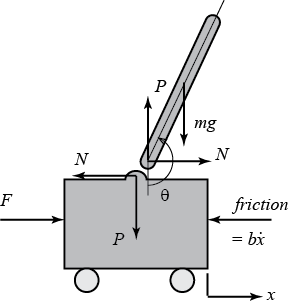
\includegraphics{pendulum2.png}

The equation for the cartpole problem is nonlinear in nature, but it has
been shown through robust control theory that a linear version of the
equation of the form \(\dot{x} = Ax+Bu\) can be solved by a linear
controller. Let us assume that we are interested in minimizing cart
stray from the center, and pendulum falling. It turns out that typical
techniques - open loop control, PID control, root locus, etc. is not
suitable for stabilizing both the cart position (keep near center) or
the pole angle (keep vertical). The solution to this question is a
linear quadratic controller, but we won't be using the solution at the
moment.

    \subsubsection{Setup Environment for Function
Approximation}\label{setup-environment-for-function-approximation}

    \begin{Verbatim}[commandchars=\\\{\}]
{\color{incolor}In [{\color{incolor}2}]:} \PY{k+kn}{import} \PY{n+nn}{gym}
        \PY{k+kn}{import} \PY{n+nn}{numpy} \PY{k+kn}{as} \PY{n+nn}{np}
        \PY{k+kn}{import} \PY{n+nn}{matplotlib.pyplot} \PY{k+kn}{as} \PY{n+nn}{plt}
        
        \PY{c+c1}{\PYZsh{} Create the CartPole game environment}
        \PY{n}{env} \PY{o}{=} \PY{n}{gym}\PY{o}{.}\PY{n}{make}\PY{p}{(}\PY{l+s+s1}{\PYZsq{}}\PY{l+s+s1}{CartPole\PYZhy{}v0}\PY{l+s+s1}{\PYZsq{}}\PY{p}{)}
        \PY{n}{state} \PY{o}{=} \PY{n}{env}\PY{o}{.}\PY{n}{reset}\PY{p}{(}\PY{p}{)}
\end{Verbatim}

    \begin{Verbatim}[commandchars=\\\{\}]
\textcolor{ansi-yellow}{WARN: gym.spaces.Box autodetected dtype as <type 'numpy.float32'>. Please provide explicit dtype.}

    \end{Verbatim}

    \paragraph{Demonstrate your understanding of the
simulation}\label{demonstrate-your-understanding-of-the-simulation}

For OpenAI's CartPole-v0 environment, - describe the reward system -
describe the each state variable (observation space) - describe the
action space

    Ans: Reward System - The environment gives us 1 reward for each state of
valid existence, including the final state. As soon as the cartpole
falls below 12 degrees on either side or goes out of screen on either
side, the episode ends in failure. The episode also ends when 200 steps
are taken without failure.

State Variable - The state variable consists of a 4 length vector
composed of the following continuous variables - * Cart Position : -2.4
to +2.4 * Cart Velocity : -inf to +inf * Pole angle : -41.8 to +41.8
degrees * Pole velocity at its tip : -inf to +inf

Action Space - The agent can take 2 action - * 0 - Push cart to the left
* 1 - Push cart to the right

    \subsubsection{Write a Deep Neural Network class that creates a dense
network of a desired
architecture}\label{write-a-deep-neural-network-class-that-creates-a-dense-network-of-a-desired-architecture}

In this problem we will create neural network that is our function that
takes states to q-values: \(q=f(x)\). While any function approximator
could be used (i.e. Chebyshev functions, taylor series polynomials),
neural networks offer a most general form of 1st-order smooth function
(though comprising of trivial small activation functions means that
complex functions require a significant amount of weights to identify).

Create a class for a QNetwork that uses PyTorch to create a fully
connected sequential neural network, of the following properties: -
solver: Adam

\begin{itemize}
\item
  input and hidden layer activation function: tanh
\item
  output activation function: linear
\item
  loss: mse
\item
  learning\_rate: variable
\item
  decay\_rate: variable
\item
  hidden\_state sizes: variable
\item
  state and action sizes: variable
\end{itemize}

    \begin{Verbatim}[commandchars=\\\{\}]
{\color{incolor}In [{\color{incolor}33}]:} \PY{k+kn}{import} \PY{n+nn}{torch}
         \PY{k+kn}{from} \PY{n+nn}{torch.autograd} \PY{k+kn}{import} \PY{n}{Variable}
         \PY{k+kn}{import} \PY{n+nn}{torch.nn} \PY{k+kn}{as} \PY{n+nn}{nn}
         \PY{k+kn}{import} \PY{n+nn}{torch.nn.functional} \PY{k+kn}{as} \PY{n+nn}{F}
         \PY{k+kn}{import} \PY{n+nn}{torch.optim} \PY{k+kn}{as} \PY{n+nn}{optim}
         \PY{k+kn}{import} \PY{n+nn}{torchvision.transforms} \PY{k+kn}{as} \PY{n+nn}{transforms}
         
         \PY{k}{def} \PY{n+nf}{toVar}\PY{p}{(}\PY{n}{x}\PY{p}{)}\PY{p}{:}
             \PY{n}{x} \PY{o}{=} \PY{n}{torch}\PY{o}{.}\PY{n}{from\PYZus{}numpy}\PY{p}{(}\PY{n}{x}\PY{p}{)}\PY{o}{.}\PY{n}{float}\PY{p}{(}\PY{p}{)}
             \PY{n}{x} \PY{o}{=} \PY{n}{Variable}\PY{p}{(}\PY{n}{x}\PY{p}{)}
             \PY{k}{return} \PY{n}{x}
         
         \PY{k}{def} \PY{n+nf}{toNp}\PY{p}{(}\PY{n}{var}\PY{p}{)}\PY{p}{:}
             \PY{k}{return} \PY{n}{var}\PY{o}{.}\PY{n}{data}\PY{o}{.}\PY{n}{numpy}\PY{p}{(}\PY{p}{)}
         
         \PY{k}{class} \PY{n+nc}{QNetwork}\PY{p}{(}\PY{n}{nn}\PY{o}{.}\PY{n}{Module}\PY{p}{)}\PY{p}{:}
         \PY{c+c1}{\PYZsh{} Define your network here       }
             \PY{k}{def} \PY{n+nf}{\PYZus{}\PYZus{}init\PYZus{}\PYZus{}}\PY{p}{(}\PY{n+nb+bp}{self}\PY{p}{,} \PY{n}{learning\PYZus{}rate}\PY{p}{,} \PY{n}{state\PYZus{}size}\PY{p}{,} \PY{n}{action\PYZus{}size}\PY{p}{,} \PY{n}{hidden\PYZus{}size}\PY{p}{,} \PY{n}{alpha\PYZus{}decay}\PY{p}{)}\PY{p}{:}
                 \PY{n+nb}{super}\PY{p}{(}\PY{n}{QNetwork}\PY{p}{,} \PY{n+nb+bp}{self}\PY{p}{)}\PY{o}{.}\PY{n}{\PYZus{}\PYZus{}init\PYZus{}\PYZus{}}\PY{p}{(}\PY{p}{)}
                 \PY{n+nb+bp}{self}\PY{o}{.}\PY{n}{layer1} \PY{o}{=} \PY{n}{nn}\PY{o}{.}\PY{n}{Linear}\PY{p}{(}\PY{n}{state\PYZus{}size}\PY{p}{,} \PY{n}{hidden\PYZus{}size}\PY{p}{)}
                 \PY{n+nb+bp}{self}\PY{o}{.}\PY{n}{layer2} \PY{o}{=} \PY{n}{nn}\PY{o}{.}\PY{n}{Linear}\PY{p}{(}\PY{n}{hidden\PYZus{}size}\PY{p}{,} \PY{n}{hidden\PYZus{}size}\PY{p}{)}
                 \PY{n+nb+bp}{self}\PY{o}{.}\PY{n}{layer3} \PY{o}{=} \PY{n}{nn}\PY{o}{.}\PY{n}{Linear}\PY{p}{(}\PY{n}{hidden\PYZus{}size}\PY{p}{,} \PY{n}{action\PYZus{}size}\PY{p}{)}
                 
                 \PY{c+c1}{\PYZsh{} Adam optimizer}
                 \PY{n+nb+bp}{self}\PY{o}{.}\PY{n}{optimizer} \PY{o}{=} \PY{n}{optim}\PY{o}{.}\PY{n}{Adam}\PY{p}{(}\PY{n+nb+bp}{self}\PY{o}{.}\PY{n}{parameters}\PY{p}{(}\PY{p}{)}\PY{p}{,} \PY{n}{lr}\PY{o}{=}\PY{n}{learning\PYZus{}rate}\PY{p}{)}
                 
                 \PY{c+c1}{\PYZsh{} LR Scheduler}
                 \PY{n+nb+bp}{self}\PY{o}{.}\PY{n}{scheduler} \PY{o}{=} \PY{n}{optim}\PY{o}{.}\PY{n}{lr\PYZus{}scheduler}\PY{o}{.}\PY{n}{StepLR}\PY{p}{(}\PY{n+nb+bp}{self}\PY{o}{.}\PY{n}{optimizer}\PY{p}{,} \PY{n}{step\PYZus{}size}\PY{o}{=}\PY{l+m+mi}{500}\PY{p}{,} \PY{n}{gamma}\PY{o}{=}\PY{n}{alpha\PYZus{}decay}\PY{p}{)}
                 
                 \PY{c+c1}{\PYZsh{} Mean squared error loss}
                 \PY{n+nb+bp}{self}\PY{o}{.}\PY{n}{criterion} \PY{o}{=} \PY{n}{nn}\PY{o}{.}\PY{n}{MSELoss}\PY{p}{(}\PY{p}{)}
                 
             \PY{k}{def} \PY{n+nf}{forward}\PY{p}{(}\PY{n+nb+bp}{self}\PY{p}{,} \PY{n}{x}\PY{p}{)}\PY{p}{:}
                 \PY{n}{x} \PY{o}{=} \PY{n}{F}\PY{o}{.}\PY{n}{tanh}\PY{p}{(}\PY{n+nb+bp}{self}\PY{o}{.}\PY{n}{layer1}\PY{p}{(}\PY{n}{x}\PY{p}{)}\PY{p}{)}
                 \PY{n}{x} \PY{o}{=} \PY{n}{F}\PY{o}{.}\PY{n}{tanh}\PY{p}{(}\PY{n+nb+bp}{self}\PY{o}{.}\PY{n}{layer2}\PY{p}{(}\PY{n}{x}\PY{p}{)}\PY{p}{)}
                 \PY{n}{x} \PY{o}{=} \PY{n+nb+bp}{self}\PY{o}{.}\PY{n}{layer3}\PY{p}{(}\PY{n}{x}\PY{p}{)}
                 \PY{k}{return} \PY{n}{x}
             
             \PY{k}{def} \PY{n+nf}{run\PYZus{}optimize}\PY{p}{(}\PY{n+nb+bp}{self}\PY{p}{,} \PY{n}{inputs}\PY{p}{,} \PY{n}{targets}\PY{p}{,} \PY{n}{mask}\PY{p}{)}\PY{p}{:}
                 \PY{n+nb+bp}{self}\PY{o}{.}\PY{n}{optimizer}\PY{o}{.}\PY{n}{zero\PYZus{}grad}\PY{p}{(}\PY{p}{)}
                 \PY{n}{outputs} \PY{o}{=} \PY{n+nb+bp}{self}\PY{p}{(}\PY{n}{inputs}\PY{p}{)}
                 \PY{n+nb+bp}{self}\PY{o}{.}\PY{n}{loss} \PY{o}{=} \PY{n+nb+bp}{self}\PY{o}{.}\PY{n}{criterion}\PY{p}{(}\PY{n}{outputs}\PY{p}{,} \PY{n}{targets}\PY{p}{)}
                 \PY{n+nb+bp}{self}\PY{o}{.}\PY{n}{loss}\PY{o}{.}\PY{n}{backward}\PY{p}{(}\PY{p}{)}
                 \PY{n+nb+bp}{self}\PY{o}{.}\PY{n}{optimizer}\PY{o}{.}\PY{n}{step}\PY{p}{(}\PY{p}{)}
                 \PY{n+nb+bp}{self}\PY{o}{.}\PY{n}{scheduler}\PY{o}{.}\PY{n}{step}\PY{p}{(}\PY{p}{)}
             
             \PY{k}{def} \PY{n+nf}{copyWeights}\PY{p}{(}\PY{n+nb+bp}{self}\PY{p}{,} \PY{n}{other}\PY{p}{)}\PY{p}{:}
                 \PY{n+nb+bp}{self}\PY{o}{.}\PY{n}{load\PYZus{}state\PYZus{}dict}\PY{p}{(}\PY{n}{other}\PY{o}{.}\PY{n}{state\PYZus{}dict}\PY{p}{(}\PY{p}{)}\PY{p}{)}
\end{Verbatim}

    \paragraph{Write a Replay class that includes all the functionality of a
replay
buffer}\label{write-a-replay-class-that-includes-all-the-functionality-of-a-replay-buffer}

The replay buffer should kept to some maximum size (10000), allow adding
of samples and returning of samples at random from the buffer. Each
sample (or experience) is formed as (state, action, reward, next\_state,
done). The replay buffer should also be able to generate a minibatch.
The generate\_minibatch method should take in DQN, targetDQN, selected
batch\_size, and return the states present in the minibatch and the
target Q values for those states.

    \begin{Verbatim}[commandchars=\\\{\}]
{\color{incolor}In [{\color{incolor}35}]:} \PY{k+kn}{import} \PY{n+nn}{random}
         
         \PY{k}{class} \PY{n+nc}{Replay}\PY{p}{(}\PY{n+nb}{object}\PY{p}{)}\PY{p}{:}
         \PY{c+c1}{\PYZsh{} Replay should also have an initialize method which creates a minimum buffer for }
         \PY{c+c1}{\PYZsh{} the initial episodes to generate minibatches.}
             \PY{k}{def} \PY{n+nf}{\PYZus{}\PYZus{}init\PYZus{}\PYZus{}}\PY{p}{(}\PY{n+nb+bp}{self}\PY{p}{,} \PY{n}{max\PYZus{}size}\PY{p}{)}\PY{p}{:}
                 \PY{n+nb+bp}{self}\PY{o}{.}\PY{n}{buffer} \PY{o}{=} \PY{p}{[}\PY{p}{]}
                 \PY{n+nb+bp}{self}\PY{o}{.}\PY{n}{capacity} \PY{o}{=} \PY{n}{max\PYZus{}size}
                 \PY{n+nb+bp}{self}\PY{o}{.}\PY{n}{position} \PY{o}{=} \PY{l+m+mi}{0}
                 
             \PY{k}{def} \PY{n+nf}{add\PYZus{}exp}\PY{p}{(}\PY{n+nb+bp}{self}\PY{p}{,} \PY{n}{state}\PY{p}{,} \PY{n}{action}\PY{p}{,} \PY{n}{reward}\PY{p}{,} \PY{n}{next\PYZus{}state}\PY{p}{,} \PY{n}{done}\PY{p}{)}\PY{p}{:}
                 \PY{k}{if} \PY{n+nb}{len}\PY{p}{(}\PY{n+nb+bp}{self}\PY{o}{.}\PY{n}{buffer}\PY{p}{)} \PY{o}{\PYZlt{}} \PY{n+nb+bp}{self}\PY{o}{.}\PY{n}{capacity}\PY{p}{:}
                     \PY{n+nb+bp}{self}\PY{o}{.}\PY{n}{buffer}\PY{o}{.}\PY{n}{append}\PY{p}{(}\PY{n+nb+bp}{None}\PY{p}{)}
                 \PY{n+nb+bp}{self}\PY{o}{.}\PY{n}{buffer}\PY{p}{[}\PY{n+nb+bp}{self}\PY{o}{.}\PY{n}{position}\PY{p}{]} \PY{o}{=} \PY{p}{(}\PY{n}{np}\PY{o}{.}\PY{n}{asarray}\PY{p}{(}\PY{n}{state}\PY{p}{)}\PY{p}{,} \PY{n}{action}\PY{p}{,} \PY{n}{reward}\PY{p}{,} \PY{n}{np}\PY{o}{.}\PY{n}{asarray}\PY{p}{(}\PY{n}{next\PYZus{}state}\PY{p}{)}\PY{p}{,} \PY{n}{done}\PY{p}{)}
                 \PY{n+nb+bp}{self}\PY{o}{.}\PY{n}{position} \PY{o}{=} \PY{p}{(}\PY{n+nb+bp}{self}\PY{o}{.}\PY{n}{position}\PY{o}{+}\PY{l+m+mi}{1}\PY{p}{)}\PY{o}{\PYZpc{}}\PY{k}{self}.capacity
             
             \PY{k}{def} \PY{n+nf}{initialize}\PY{p}{(}\PY{n+nb+bp}{self}\PY{p}{,} \PY{n}{init\PYZus{}length}\PY{p}{,} \PY{n}{envir}\PY{p}{)}\PY{p}{:}
                 \PY{n}{state} \PY{o}{=} \PY{n}{envir}\PY{o}{.}\PY{n}{reset}\PY{p}{(}\PY{p}{)}
                 \PY{k}{while}\PY{p}{(}\PY{n+nb}{len}\PY{p}{(}\PY{n+nb+bp}{self}\PY{o}{.}\PY{n}{buffer}\PY{p}{)}\PY{o}{\PYZlt{}}\PY{n}{init\PYZus{}length}\PY{p}{)}\PY{p}{:}
                     \PY{n}{state} \PY{o}{=} \PY{n}{envir}\PY{o}{.}\PY{n}{env}\PY{o}{.}\PY{n}{state}
                     \PY{n}{action} \PY{o}{=} \PY{n}{envir}\PY{o}{.}\PY{n}{action\PYZus{}space}\PY{o}{.}\PY{n}{sample}\PY{p}{(}\PY{p}{)}
                     \PY{n}{next\PYZus{}state}\PY{p}{,} \PY{n}{reward}\PY{p}{,} \PY{n}{done}\PY{p}{,} \PY{n}{\PYZus{}} \PY{o}{=} \PY{n}{envir}\PY{o}{.}\PY{n}{step}\PY{p}{(}\PY{n}{action}\PY{p}{)}
                     \PY{n+nb+bp}{self}\PY{o}{.}\PY{n}{add\PYZus{}exp}\PY{p}{(}\PY{n}{state}\PY{p}{,} \PY{n}{action}\PY{p}{,} \PY{n}{reward}\PY{p}{,} \PY{n}{next\PYZus{}state}\PY{p}{,} \PY{n}{done}\PY{p}{)}
                     \PY{k}{if} \PY{n}{done}\PY{p}{:}
                         \PY{n}{state} \PY{o}{=} \PY{n}{envir}\PY{o}{.}\PY{n}{reset}\PY{p}{(}\PY{p}{)}
                     \PY{k}{else}\PY{p}{:}
                         \PY{n}{state} \PY{o}{=} \PY{n}{next\PYZus{}state}
             
             \PY{k}{def} \PY{n+nf}{sample}\PY{p}{(}\PY{n+nb+bp}{self}\PY{p}{,} \PY{n}{batch\PYZus{}size}\PY{p}{)}\PY{p}{:}
                 \PY{k}{return} \PY{n}{random}\PY{o}{.}\PY{n}{sample}\PY{p}{(}\PY{n+nb+bp}{self}\PY{o}{.}\PY{n}{buffer}\PY{p}{,} \PY{n}{batch\PYZus{}size}\PY{p}{)}
                     
             \PY{k}{def} \PY{n+nf}{generate\PYZus{}minibatch}\PY{p}{(}\PY{n+nb+bp}{self}\PY{p}{,} \PY{n}{DQN}\PY{p}{,} \PY{n}{targetDQN}\PY{p}{,} \PY{n}{batch\PYZus{}size}\PY{p}{,} \PY{n}{gamma}\PY{p}{)}\PY{p}{:}
                 \PY{n}{states} \PY{o}{=} \PY{p}{[}\PY{p}{]}
                 \PY{n}{target\PYZus{}qvalues} \PY{o}{=} \PY{p}{[}\PY{p}{]}
                 \PY{n}{actions} \PY{o}{=} \PY{n}{np}\PY{o}{.}\PY{n}{ones}\PY{p}{(}\PY{p}{(}\PY{n}{batch\PYZus{}size}\PY{p}{,}\PY{l+m+mi}{2}\PY{p}{)}\PY{p}{)}
                 \PY{n}{samples} \PY{o}{=} \PY{n+nb+bp}{self}\PY{o}{.}\PY{n}{sample}\PY{p}{(}\PY{n}{batch\PYZus{}size}\PY{p}{)}
                 \PY{n}{counter} \PY{o}{=} \PY{l+m+mi}{0}
                 \PY{k}{for} \PY{n}{state}\PY{p}{,} \PY{n}{action}\PY{p}{,} \PY{n}{reward}\PY{p}{,} \PY{n}{next\PYZus{}state}\PY{p}{,} \PY{n}{done} \PY{o+ow}{in} \PY{n}{samples}\PY{p}{:}
                     \PY{c+c1}{\PYZsh{} if done then qvalue is the reward itself}
                     \PY{c+c1}{\PYZsh{} else it is reward+gamma*max(targetQ(s\PYZsq{}))}
                     \PY{n}{max\PYZus{}qsa} \PY{o}{=} \PY{n}{reward}
                     \PY{k}{if} \PY{o+ow}{not} \PY{n}{done}\PY{p}{:}
                         \PY{n}{target\PYZus{}q} \PY{o}{=} \PY{n}{toNp}\PY{p}{(}\PY{n}{targetDQN}\PY{p}{(}\PY{n}{toVar}\PY{p}{(}\PY{n}{next\PYZus{}state}\PY{p}{)}\PY{p}{)}\PY{p}{)}
                         \PY{n}{max\PYZus{}qsa} \PY{o}{+}\PY{o}{=} \PY{n}{gamma}\PY{o}{*}\PY{n+nb}{max}\PY{p}{(}\PY{n}{target\PYZus{}q}\PY{p}{)}
                     
                     \PY{c+c1}{\PYZsh{} qvalues for the action taken need to be optimized}
                     \PY{n}{y} \PY{o}{=} \PY{n}{toNp}\PY{p}{(}\PY{n}{DQN}\PY{p}{(}\PY{n}{toVar}\PY{p}{(}\PY{n}{state}\PY{p}{)}\PY{p}{)}\PY{p}{)}
                     \PY{n}{y}\PY{p}{[}\PY{n}{action}\PY{p}{]} \PY{o}{=} \PY{n}{max\PYZus{}qsa}
                     \PY{n}{actions}\PY{p}{[}\PY{n}{counter}\PY{p}{,}\PY{n}{action}\PY{p}{]} \PY{o}{=} \PY{l+m+mi}{1}
                     \PY{n}{counter}\PY{o}{+}\PY{o}{=}\PY{l+m+mi}{1}
                     \PY{n}{states}\PY{o}{.}\PY{n}{append}\PY{p}{(}\PY{n}{state}\PY{p}{)}
                     \PY{n}{target\PYZus{}qvalues}\PY{o}{.}\PY{n}{append}\PY{p}{(}\PY{n}{y}\PY{p}{)}
                     
                     
                 \PY{n}{states} \PY{o}{=} \PY{n}{np}\PY{o}{.}\PY{n}{asarray}\PY{p}{(}\PY{n}{states}\PY{p}{)}
                 \PY{n}{target\PYZus{}qvalues} \PY{o}{=} \PY{n}{np}\PY{o}{.}\PY{n}{asarray}\PY{p}{(}\PY{n}{target\PYZus{}qvalues}\PY{p}{)}
                 \PY{k}{return} \PY{n}{states}\PY{p}{,} \PY{n}{actions}\PY{p}{,} \PY{n}{target\PYZus{}qvalues}
                         
\end{Verbatim}

    Write a function that creates a minibatch from a buffer

    \subsubsection{Perform Function
Approximation}\label{perform-function-approximation}

Initialize DQN networks and Replay objects

    \begin{Verbatim}[commandchars=\\\{\}]
{\color{incolor}In [{\color{incolor}51}]:} \PY{c+c1}{\PYZsh{} Initialize DQN}
         \PY{c+c1}{\PYZsh{} Play around with your learning rate, alpha decay and hidden layer units }
         \PY{c+c1}{\PYZsh{} Two layers with a small number of units should be enough}
         \PY{n}{learning\PYZus{}rate} \PY{o}{=} \PY{l+m+mf}{0.0008}
         \PY{n}{state\PYZus{}size} \PY{o}{=} \PY{n}{env}\PY{o}{.}\PY{n}{observation\PYZus{}space}\PY{o}{.}\PY{n}{shape}\PY{p}{[}\PY{l+m+mi}{0}\PY{p}{]}
         \PY{n}{action\PYZus{}size} \PY{o}{=} \PY{n}{env}\PY{o}{.}\PY{n}{action\PYZus{}space}\PY{o}{.}\PY{n}{n}
         \PY{n}{hidden\PYZus{}size} \PY{o}{=} \PY{l+m+mi}{100}
         \PY{n}{alpha\PYZus{}decay} \PY{o}{=} \PY{l+m+mf}{0.08}
         \PY{n}{DQN} \PY{o}{=} \PY{n}{QNetwork}\PY{p}{(}\PY{n}{learning\PYZus{}rate}\PY{p}{,} \PY{n}{state\PYZus{}size}\PY{p}{,} \PY{n}{action\PYZus{}size}\PY{p}{,} \PY{n}{hidden\PYZus{}size}\PY{p}{,} \PY{n}{alpha\PYZus{}decay}\PY{p}{)}
         \PY{n}{targetDQN} \PY{o}{=} \PY{n}{QNetwork}\PY{p}{(}\PY{n}{learning\PYZus{}rate}\PY{p}{,} \PY{n}{state\PYZus{}size}\PY{p}{,} \PY{n}{action\PYZus{}size}\PY{p}{,} \PY{n}{hidden\PYZus{}size}\PY{p}{,} \PY{n}{alpha\PYZus{}decay}\PY{p}{)}
         
         \PY{c+c1}{\PYZsh{} set targetDQN weights to DQN weights}
         \PY{c+c1}{\PYZsh{} for ex. targetDQN.model.weights = DQN.model.weights (syntax given here is for representation purpose only)}
         \PY{n}{targetDQN}\PY{o}{.}\PY{n}{copyWeights}\PY{p}{(}\PY{n}{DQN}\PY{p}{)}
         
         \PY{c+c1}{\PYZsh{}\PYZsh{} Initialize Replay Buffer}
         \PY{c+c1}{\PYZsh{}\PYZsh{}\PYZsh{}\PYZsh{}\PYZsh{}\PYZsh{}\PYZsh{}\PYZsh{}\PYZsh{}\PYZsh{}\PYZsh{}\PYZsh{}\PYZsh{}\PYZsh{}\PYZsh{}\PYZsh{}\PYZsh{}\PYZsh{}\PYZsh{}\PYZsh{}\PYZsh{}\PYZsh{}\PYZsh{}\PYZsh{}\PYZsh{}\PYZsh{}\PYZsh{}\PYZsh{}\PYZsh{}\PYZsh{}\PYZsh{}\PYZsh{}\PYZsh{}\PYZsh{}\PYZsh{}}
         \PY{c+c1}{\PYZsh{}\PYZsh{} Populate the initial experience buffer}
         \PY{c+c1}{\PYZsh{}\PYZsh{}\PYZsh{}\PYZsh{}\PYZsh{}\PYZsh{}\PYZsh{}\PYZsh{}\PYZsh{}\PYZsh{}\PYZsh{}\PYZsh{}\PYZsh{}\PYZsh{}\PYZsh{}\PYZsh{}\PYZsh{}\PYZsh{}\PYZsh{}\PYZsh{}\PYZsh{}\PYZsh{}\PYZsh{}\PYZsh{}\PYZsh{}\PYZsh{}\PYZsh{}\PYZsh{}\PYZsh{}\PYZsh{}\PYZsh{}\PYZsh{}\PYZsh{}\PYZsh{}\PYZsh{}}
         
         \PY{n}{replay} \PY{o}{=} \PY{n}{Replay}\PY{p}{(}\PY{n}{max\PYZus{}size}\PY{o}{=}\PY{l+m+mi}{10000}\PY{p}{)}
         \PY{n}{replay}\PY{o}{.}\PY{n}{initialize}\PY{p}{(}\PY{n}{init\PYZus{}length}\PY{o}{=}\PY{l+m+mi}{1000}\PY{p}{,} \PY{n}{envir}\PY{o}{=}\PY{n}{env}\PY{p}{)}
\end{Verbatim}

    \paragraph{Create a function that solves the above environment using a
deep Q network that uses a minibatch
strategy.}\label{create-a-function-that-solves-the-above-environment-using-a-deep-q-network-that-uses-a-minibatch-strategy.}

Use the following parameters (these had to be derived empirically -
there is generally no trusted way of choosing the right parameter values
- i.e. gamma, number of episodes, decay rate, min\_epsilon).

Generate a graph of the average return per episode every 100 episodes.

    \begin{Verbatim}[commandchars=\\\{\}]
{\color{incolor}In [{\color{incolor}52}]:} \PY{c+c1}{\PYZsh{} Runtime parameters}
         \PY{n}{num\PYZus{}episodes} \PY{o}{=} \PY{l+m+mi}{2000}            \PY{c+c1}{\PYZsh{} max number of episodes to learn from}
         \PY{n}{gamma} \PY{o}{=} \PY{l+m+mf}{0.95}                   \PY{c+c1}{\PYZsh{} future reward discount}
         \PY{n}{max\PYZus{}steps} \PY{o}{=} \PY{l+m+mi}{2000}                \PY{c+c1}{\PYZsh{} cut off simulation after this many steps}
         \PY{n}{batch\PYZus{}size} \PY{o}{=} \PY{l+m+mi}{250}
         \PY{n}{C} \PY{o}{=} \PY{l+m+mi}{50}
         
         \PY{c+c1}{\PYZsh{} Exploration parameters}
         \PY{n}{min\PYZus{}epsilon} \PY{o}{=} \PY{l+m+mf}{0.001}             \PY{c+c1}{\PYZsh{} minimum exploration probability}
         \PY{n}{decay\PYZus{}rate} \PY{o}{=} \PY{l+m+mf}{5.0}\PY{o}{/}\PY{n}{num\PYZus{}episodes}    \PY{c+c1}{\PYZsh{} exponential decay rate for exploration prob}
         \PY{n}{returns} \PY{o}{=} \PY{n}{np}\PY{o}{.}\PY{n}{zeros}\PY{p}{(}\PY{n}{num\PYZus{}episodes}\PY{p}{)}
         
         \PY{k}{for} \PY{n}{ep} \PY{o+ow}{in} \PY{n+nb}{range}\PY{p}{(}\PY{l+m+mi}{0}\PY{p}{,} \PY{n}{num\PYZus{}episodes}\PY{p}{)}\PY{p}{:}
             \PY{n}{epsilon} \PY{o}{=} \PY{n}{min\PYZus{}epsilon} \PY{o}{+} \PY{p}{(}\PY{l+m+mf}{1.0} \PY{o}{\PYZhy{}} \PY{n}{min\PYZus{}epsilon}\PY{p}{)}\PY{o}{*}\PY{n}{np}\PY{o}{.}\PY{n}{exp}\PY{p}{(}\PY{o}{\PYZhy{}}\PY{n}{decay\PYZus{}rate}\PY{o}{*}\PY{n}{ep}\PY{p}{)}
             \PY{n}{state} \PY{o}{=} \PY{n}{env}\PY{o}{.}\PY{n}{reset}\PY{p}{(}\PY{p}{)}
             \PY{n}{total\PYZus{}reward} \PY{o}{=} \PY{l+m+mf}{0.0}
             \PY{k}{for} \PY{n}{step} \PY{o+ow}{in} \PY{n+nb}{range}\PY{p}{(}\PY{n}{max\PYZus{}steps}\PY{p}{)}\PY{p}{:}
                 \PY{c+c1}{\PYZsh{} \PYZhy{}\PYZhy{}\PYZgt{} start episode}
                 \PY{n}{q\PYZus{}sa} \PY{o}{=} \PY{n}{toNp}\PY{p}{(}\PY{n}{DQN}\PY{p}{(}\PY{n}{toVar}\PY{p}{(}\PY{n}{state}\PY{p}{)}\PY{p}{)}\PY{p}{)}
                 \PY{n}{action} \PY{o}{=} \PY{n}{np}\PY{o}{.}\PY{n}{argmax}\PY{p}{(}\PY{n}{q\PYZus{}sa}\PY{p}{)}
                 
                 \PY{c+c1}{\PYZsh{} explore/exploit and get action using DQN}
                 \PY{c+c1}{\PYZsh{} binary action space}
                 \PY{k}{if} \PY{n}{np}\PY{o}{.}\PY{n}{random}\PY{o}{.}\PY{n}{rand}\PY{p}{(}\PY{p}{)}\PY{o}{\PYZlt{}}\PY{n}{epsilon}\PY{p}{:}
                     \PY{n}{action} \PY{o}{=} \PY{n}{env}\PY{o}{.}\PY{n}{action\PYZus{}space}\PY{o}{.}\PY{n}{sample}\PY{p}{(}\PY{p}{)}
                     
                 \PY{c+c1}{\PYZsh{} perform action and record new\PYZus{}state, action, reward}
                 \PY{n}{next\PYZus{}state}\PY{p}{,} \PY{n}{reward}\PY{p}{,} \PY{n}{done}\PY{p}{,} \PY{n}{\PYZus{}} \PY{o}{=} \PY{n}{env}\PY{o}{.}\PY{n}{step}\PY{p}{(}\PY{n}{action}\PY{p}{)}
                 \PY{n}{total\PYZus{}reward} \PY{o}{+}\PY{o}{=} \PY{n}{reward}
                 
                 \PY{c+c1}{\PYZsh{} populate Replay experience buffer}
                 \PY{n}{replay}\PY{o}{.}\PY{n}{add\PYZus{}exp}\PY{p}{(}\PY{n}{state}\PY{p}{,} \PY{n}{action}\PY{p}{,} \PY{n}{reward}\PY{p}{,} \PY{n}{next\PYZus{}state}\PY{p}{,} \PY{n}{done}\PY{p}{)}
                 
                 \PY{k}{if} \PY{n}{done}\PY{p}{:}
                     \PY{k}{break}
                 \PY{k}{else}\PY{p}{:}
                     \PY{n}{state} \PY{o}{=} \PY{n}{next\PYZus{}state}
                 \PY{c+c1}{\PYZsh{} \PYZlt{}\PYZhy{}\PYZhy{} end episode}
         
             \PY{n}{returns}\PY{p}{[}\PY{n}{ep}\PY{p}{]} \PY{o}{=} \PY{n}{total\PYZus{}reward}
             \PY{c+c1}{\PYZsh{}print(returns[ep])}
         
             \PY{c+c1}{\PYZsh{} Replay}
             \PY{n}{states}\PY{p}{,} \PY{n}{actions}\PY{p}{,} \PY{n}{target\PYZus{}qvalues} \PY{o}{=} \PY{n}{replay}\PY{o}{.}\PY{n}{generate\PYZus{}minibatch}\PY{p}{(}\PY{n}{DQN}\PY{p}{,} \PY{n}{targetDQN}\PY{p}{,} \PY{n}{batch\PYZus{}size}\PY{p}{,} \PY{n}{gamma}\PY{p}{)}
             
             \PY{c+c1}{\PYZsh{} set targetDQN weights to DQN weights}
             \PY{k}{if} \PY{p}{(}\PY{n}{ep}\PY{o}{+}\PY{l+m+mi}{1}\PY{p}{)}\PY{o}{\PYZpc{}}\PY{k}{C}==0:
                 \PY{k}{print}\PY{p}{(}\PY{n}{ep}\PY{o}{+}\PY{l+m+mi}{1}\PY{p}{,} \PY{n}{returns}\PY{p}{[}\PY{n}{ep}\PY{p}{]}\PY{p}{)}
                 \PY{n}{targetDQN}\PY{o}{.}\PY{n}{copyWeights}\PY{p}{(}\PY{n}{DQN}\PY{p}{)}
             
             \PY{c+c1}{\PYZsh{} update DQN (run one epoch of training per episode with generated minibatch of states and qvalues)}
             \PY{c+c1}{\PYZsh{}for i in range(states.shape[0]):}
             \PY{c+c1}{\PYZsh{}    DQN.run\PYZus{}optimize(toVar(states[i]), toVar(target\PYZus{}qvalues[i]))}
             \PY{n}{DQN}\PY{o}{.}\PY{n}{run\PYZus{}optimize}\PY{p}{(}\PY{n}{toVar}\PY{p}{(}\PY{n}{states}\PY{p}{)}\PY{p}{,} \PY{n}{toVar}\PY{p}{(}\PY{n}{target\PYZus{}qvalues}\PY{p}{)}\PY{p}{,} \PY{n}{toVar}\PY{p}{(}\PY{n}{actions}\PY{p}{)}\PY{p}{)}        
\end{Verbatim}

    \begin{Verbatim}[commandchars=\\\{\}]
(50, 27.0)
(100, 12.0)
(150, 39.0)
(200, 33.0)
(250, 56.0)
(300, 21.0)
(350, 54.0)
(400, 90.0)
(450, 101.0)
(500, 200.0)
(550, 200.0)
(600, 200.0)
(650, 200.0)
(700, 200.0)
(750, 200.0)
(800, 200.0)
(850, 200.0)
(900, 200.0)
(950, 200.0)
(1000, 200.0)
(1050, 200.0)
(1100, 200.0)
(1150, 200.0)
(1200, 200.0)
(1250, 200.0)
(1300, 200.0)
(1350, 200.0)
(1400, 200.0)
(1450, 200.0)
(1500, 200.0)
(1550, 200.0)
(1600, 200.0)
(1650, 200.0)
(1700, 200.0)
(1750, 200.0)
(1800, 200.0)
(1850, 200.0)
(1900, 200.0)
(1950, 200.0)
(2000, 200.0)

    \end{Verbatim}

    \begin{Verbatim}[commandchars=\\\{\}]
{\color{incolor}In [{\color{incolor}53}]:} \PY{c+c1}{\PYZsh{} plot average returns}
         \PY{n}{returns\PYZus{}over\PYZus{}100\PYZus{}episodes} \PY{o}{=} \PY{p}{[}\PY{p}{]}
         \PY{n}{x} \PY{o}{=} \PY{p}{[}\PY{p}{]}
         \PY{k}{for} \PY{n}{i} \PY{o+ow}{in} \PY{n+nb}{range}\PY{p}{(}\PY{l+m+mi}{0}\PY{p}{,}\PY{n+nb}{int}\PY{p}{(}\PY{n}{num\PYZus{}episodes}\PY{o}{/}\PY{l+m+mi}{100}\PY{p}{)}\PY{p}{)}\PY{p}{:}
             \PY{n}{returns\PYZus{}over\PYZus{}100\PYZus{}episodes}\PY{o}{.}\PY{n}{append}\PY{p}{(}\PY{n+nb}{sum}\PY{p}{(}\PY{n}{returns}\PY{p}{[}\PY{l+m+mi}{100}\PY{o}{*}\PY{n}{i}\PY{p}{:}\PY{l+m+mi}{100}\PY{o}{*}\PY{p}{(}\PY{n}{i}\PY{o}{+}\PY{l+m+mi}{1}\PY{p}{)}\PY{o}{\PYZhy{}}\PY{l+m+mi}{1}\PY{p}{]}\PY{p}{)}\PY{o}{/}\PY{l+m+mi}{100}\PY{p}{)}
             \PY{n}{x}\PY{o}{.}\PY{n}{append}\PY{p}{(}\PY{p}{(}\PY{n}{i}\PY{o}{+}\PY{l+m+mi}{1}\PY{p}{)}\PY{o}{*}\PY{l+m+mi}{100}\PY{p}{)}
         \PY{n}{plt}\PY{o}{.}\PY{n}{plot}\PY{p}{(}\PY{n}{x}\PY{p}{,}\PY{n}{returns\PYZus{}over\PYZus{}100\PYZus{}episodes}\PY{p}{,}\PY{l+s+s1}{\PYZsq{}}\PY{l+s+s1}{.\PYZhy{}r}\PY{l+s+s1}{\PYZsq{}}\PY{p}{)}
         \PY{n}{plt}\PY{o}{.}\PY{n}{ylabel}\PY{p}{(}\PY{l+s+s1}{\PYZsq{}}\PY{l+s+s1}{Average Returns per Episode}\PY{l+s+s1}{\PYZsq{}}\PY{p}{)}
         \PY{n}{plt}\PY{o}{.}\PY{n}{xlabel}\PY{p}{(}\PY{l+s+s1}{\PYZsq{}}\PY{l+s+s1}{Num of Episodes}\PY{l+s+s1}{\PYZsq{}}\PY{p}{)}
         \PY{n}{plt}\PY{o}{.}\PY{n}{show}\PY{p}{(}\PY{p}{)}
             
\end{Verbatim}

    \begin{center}
    \adjustimage{max size={0.9\linewidth}{0.9\paperheight}}{output_15_0.png}
    \end{center}
    { \hspace*{\fill} \\}
    
    \begin{Verbatim}[commandchars=\\\{\}]
{\color{incolor}In [{\color{incolor}147}]:} \PY{c+c1}{\PYZsh{} DEMO FINAL NETWORK}
          \PY{k+kn}{import} \PY{n+nn}{matplotlib.pyplot} \PY{k+kn}{as} \PY{n+nn}{plt}
          \PY{o}{\PYZpc{}}\PY{k}{matplotlib} inline
          \PY{k+kn}{from} \PY{n+nn}{IPython} \PY{k+kn}{import} \PY{n}{display}
          
          \PY{k}{def} \PY{n+nf}{show\PYZus{}state}\PY{p}{(}\PY{n}{env}\PY{p}{,} \PY{n}{step}\PY{o}{=}\PY{l+m+mi}{0}\PY{p}{,} \PY{n}{info}\PY{o}{=}\PY{l+s+s2}{\PYZdq{}}\PY{l+s+s2}{\PYZdq{}}\PY{p}{)}\PY{p}{:}
              \PY{n}{plt}\PY{o}{.}\PY{n}{figure}\PY{p}{(}\PY{l+m+mi}{3}\PY{p}{)}
              \PY{n}{plt}\PY{o}{.}\PY{n}{clf}\PY{p}{(}\PY{p}{)}
              \PY{n}{plt}\PY{o}{.}\PY{n}{imshow}\PY{p}{(}\PY{n}{env}\PY{o}{.}\PY{n}{render}\PY{p}{(}\PY{n}{mode}\PY{o}{=}\PY{l+s+s1}{\PYZsq{}}\PY{l+s+s1}{rgb\PYZus{}array}\PY{l+s+s1}{\PYZsq{}}\PY{p}{)}\PY{p}{)}
              \PY{n}{plt}\PY{o}{.}\PY{n}{axis}\PY{p}{(}\PY{l+s+s1}{\PYZsq{}}\PY{l+s+s1}{off}\PY{l+s+s1}{\PYZsq{}}\PY{p}{)}
          
              \PY{n}{display}\PY{o}{.}\PY{n}{clear\PYZus{}output}\PY{p}{(}\PY{n}{wait}\PY{o}{=}\PY{n+nb+bp}{True}\PY{p}{)}
              \PY{n}{display}\PY{o}{.}\PY{n}{display}\PY{p}{(}\PY{n}{plt}\PY{o}{.}\PY{n}{gcf}\PY{p}{(}\PY{p}{)}\PY{p}{)}
          
          
          \PY{n}{env} \PY{o}{=} \PY{n}{gym}\PY{o}{.}\PY{n}{make}\PY{p}{(}\PY{l+s+s1}{\PYZsq{}}\PY{l+s+s1}{CartPole\PYZhy{}v0}\PY{l+s+s1}{\PYZsq{}}\PY{p}{)}
          \PY{n}{env}\PY{o}{.}\PY{n}{reset}\PY{p}{(}\PY{p}{)}
          \PY{c+c1}{\PYZsh{} Take one random step to get the pole and cart moving}
          \PY{n}{state}\PY{p}{,} \PY{n}{reward}\PY{p}{,} \PY{n}{done}\PY{p}{,} \PY{n}{\PYZus{}} \PY{o}{=} \PY{n}{env}\PY{o}{.}\PY{n}{step}\PY{p}{(}\PY{n}{env}\PY{o}{.}\PY{n}{action\PYZus{}space}\PY{o}{.}\PY{n}{sample}\PY{p}{(}\PY{p}{)}\PY{p}{)}
          \PY{n}{state} \PY{o}{=} \PY{n}{np}\PY{o}{.}\PY{n}{reshape}\PY{p}{(}\PY{n}{state}\PY{p}{,} \PY{p}{[}\PY{l+m+mi}{1}\PY{p}{,} \PY{n}{state}\PY{o}{.}\PY{n}{size}\PY{p}{]}\PY{p}{)}
          \PY{n}{total\PYZus{}reward} \PY{o}{=} \PY{l+m+mi}{0}
          \PY{k}{for} \PY{n}{i} \PY{o+ow}{in} \PY{n+nb}{range}\PY{p}{(}\PY{l+m+mi}{0}\PY{p}{,} \PY{n}{max\PYZus{}steps}\PY{p}{)}\PY{p}{:}
              \PY{c+c1}{\PYZsh{}env.render()}
              \PY{n}{show\PYZus{}state}\PY{p}{(}\PY{n}{env}\PY{p}{,}\PY{n}{i}\PY{p}{)}
              
              \PY{n}{Qs} \PY{o}{=} \PY{n}{toNp}\PY{p}{(}\PY{n}{DQN}\PY{p}{(}\PY{n}{toVar}\PY{p}{(}\PY{n}{state}\PY{p}{)}\PY{p}{)}\PY{p}{)}
              \PY{c+c1}{\PYZsh{} Get action from Q\PYZhy{}network}
              \PY{c+c1}{\PYZsh{} Qs = output of DQN.model when state is passed in}
              \PY{n}{action} \PY{o}{=} \PY{n}{np}\PY{o}{.}\PY{n}{argmax}\PY{p}{(}\PY{n}{Qs}\PY{p}{)}
              
              \PY{c+c1}{\PYZsh{} Take action, get new state and reward}
              \PY{n}{next\PYZus{}state}\PY{p}{,} \PY{n}{reward}\PY{p}{,} \PY{n}{done}\PY{p}{,} \PY{n}{\PYZus{}} \PY{o}{=} \PY{n}{env}\PY{o}{.}\PY{n}{step}\PY{p}{(}\PY{n}{action}\PY{p}{)}
              \PY{n}{total\PYZus{}reward} \PY{o}{+}\PY{o}{=} \PY{n}{reward}
          
              \PY{k}{if} \PY{n}{done}\PY{p}{:}
                  \PY{c+c1}{\PYZsh{}env.close()}
                  \PY{k}{break}
              \PY{k}{else}\PY{p}{:}
                  \PY{n}{state} \PY{o}{=} \PY{n}{np}\PY{o}{.}\PY{n}{reshape}\PY{p}{(}\PY{n}{next\PYZus{}state}\PY{p}{,} \PY{p}{[}\PY{l+m+mi}{1}\PY{p}{,} \PY{n}{state}\PY{o}{.}\PY{n}{size}\PY{p}{]}\PY{p}{)}
\end{Verbatim}

    \begin{center}
    \adjustimage{max size={0.9\linewidth}{0.9\paperheight}}{output_16_0.png}
    \end{center}
    { \hspace*{\fill} \\}
    
    \begin{center}
    \adjustimage{max size={0.9\linewidth}{0.9\paperheight}}{output_16_1.png}
    \end{center}
    { \hspace*{\fill} \\}
    

    % Add a bibliography block to the postdoc
    
    
    
    \end{document}
